\chapter{Preface}

Like any major research endeavor, this thesis certainly didn't start anywhere near
where it ended.
Most of the credit for the genesis for this thesis needs to be given to 
Sivan Toledo, 4X6IZ, from Tel-Aviv University. In 2012 he wrote an article in the
amateur radio QEX technical journal where he explored improving the soundcard 
digital signal processing modem used for amateur packet radio by passing the 
original signals through a series of band-pass filters \cite{sevanhighperf}. 
His improvements were
commendable, and his article was very well written, but what bothered me was that 
more than three decades after the inception of amateur packet radio,
we are still seeing
measurable improvement in the modems we use for the original modulation techniques.

This thesis started with me wanting to tear apart the current state of the various
Bell 202 modems used in amateur radio, build a quantitative model of the kinds of
interference and distortion that each modem handled well, and hopefully design
a new signal processing algorithm that showed immunity to the most common forms of
interference on real-world channels. Sevan's work in JAVA showed promise, but 
while his library is useful on desktop computers and Android devices, it left 
out in the cold the many different 8, 16, and 32 bit fixed-point microcontrollers
that are often used for embedded modems in amateur radio projects.

As I started to examine the specifications for the various network layers used
in the amateur Automatic Packet Reporting System (namely Bell 202, AX.25, and
APRS), I grew increasingly shocked and confused when I kept finding that the
documentation I was looking for was poorly written or simply didn't exist. 
Protocol specifications would identify variables critical for network performance,
and then never give guidance on what the actual value should be.
Many of the documents
on the expected behavior for network nodes consist solely of console commands
to be run on specific pieces of discontinued hardware instead of actual protocol
behavior.
Most articles discussing aspects of the network disagreed with 
other documentation on specific details,
and was often internally inconsistent as well.

The final turning point was an interview in March, 2014 with Scott Miller, the
designer for Open Trackers, 
which are one of the more popular lines of contemporary modems used in the APRS
network.
I brought a laundry list of inconsistencies from the network specs and he
explained how much effort he had put into reverse engineering the existing 
hardware. It was an eye-opening conversation that drove home how much the 
amateur packet network has grown haphazardly over the past three decades into
a jumble of band-aids applied upon band-aids.

I realized that the most important academic research on the topic of APRS isn't
how to squeeze out another incremental improvement in one of the modem DSP
algorithms, but an over-arching prolegomenon on the entire network stack as it 
actually exists today. The existing documentation clearly falls short, and
much of the institutional knowledge that I've been able to draw on during 
my research is coming from the ``old guard" of the hobby, which leaves us exposed
to the labor intensive requirement of newcomers to the network to 
reverse engineer the existing network before they can participate.

Ideally, this document would be able to stand by itself as a complete 
``implementer's guide to APRS" from the physical layer all the way up to high level
aggregate network behavior, but the scope of reverse engineering that much
behavior, documenting it, and then verifying the documentation quickly becomes
monumental. 
It is my hope that this document does at least identify the most glaring 
short-falls in the current documentation and network design, and gives answers to
the questions that can be answered while staying within the scope of this survey.

For every identified problem which is answered in this paper, there
are twice as many unanswered questions which each warrant being considered 
as a thesis of their own.


\chapter{Introduction}

The Automatic Packet Reporting System (APRS) is an amateur radio packet
network designed to provide each participating node a local view of the 
tactical environment based on each node beaconing its current status
and advertising any other local resources known to exist.

Exactly what types of resources should be advertised on a local APRS
network is left to the discretion of the local network coordinators, but
a typical APRS network would advertise information such as:
\begin{itemize}
\item The location of amateur radio operators and what frequencies they are using for voice communications.
\item The location, frequency, and access information for voice repeaters.
\item The location and status of APRS digital repeater nodes.
\item The location and access information for other packet networks such as BBSes, Winlink nodes, or open Internet access points.
\item The location and status of useful facilities such as rest stops or resupply points for food and water.
\item Telemetry from sensors such as weather stations or remote site monitoring equipment.
\item Short real-time messages and announcements directed at other amateur radio operators.
\end{itemize} 

Despite these flexible capabilities, 
and much to the chagrin of many of the original designers of APRS, 
the vast majority of user traffic on the APRS network consists solely of 
real-time automatic vehicle tracking (AVT).
Fittingly, it follows that one of the hotbeds for APRS network congestion
is the Los Angeles basin, 
due to its bowl-shaped geography and unusually high population density. \cite{bobfixla}
When discussing specifics of the APRS network, such as how often to send traffic
or how many hops to route it over, LA invariably comes up as a counter-example
that under-cuts any specific guidance on what to expect from the network.

The author is more interested in being able to make concise statements about 
APRS in general than construct an entirely exhaustive analysis, 
so the reader need only appreciate that places like LA are the exception to the rules.
Any readers operating in the LA basin have the author's heart-felt condolences,
but need look elsewhere for definitive guidance on operating in such a unique
part of the APRS network.

\section{History of APRS}

APRS was created as an evolution of the AX.25 packet networks
built throughout the amateur community during the 1980s and 1990s and 
the Connectionless Emergency Traffic System (CETS) built by 
Bob Bruninga during the early 1980s to map Navy position reports.

Near-ubiquitous access to the Internet caused the decline in local BBS 
systems and AX.25 TCP/IP networks during the 1990s, but APRS has 
continued to enjoy a growing user-base due to it filling a unique 
application of amateur packet radio to local short-lived communication.
The 1200 baud Bell 202 modems used for AX.25 are often bemoaned for having
such a low data rate, but proves to be plenty of bandwidth for the short periodic
text messages involved in APRS.

APRS supports basic communication between stations via node to node 
text messages and comment field status updates, but should not be 
considered a communications network to an end, but a way to be made aware
of the other assets in the local area made available to support amateur 
radio operations.

Since APRS is built upon the relatively slow 
1200bps AX.25 VHF packet
network and the channel sharing concepts developed for the ALOHAnet at
the University of Hawaii, the amount of 
traffic and the number of stations that it is possible to successfully 
support on a single regional network is severely limited. 
A typical APRS network is considered successful if a single node
can use it to discover the 60 closest other assets on the network in a
10-30 minute time frame. Trying to advertise information beyond this
``ALOHA circle" consisting of the 60 closest stations exceeds the 
operational objective of the APRS network and usually proves to only be 
detrimental to the network and other users as network throughput is 
consumed by advertisements for 
resources beyond the radius of interest for the local operator.

\section{Physical Topology and Hardware}

A typical APRS network consists of three types of stations:
\begin{itemize}
	\item Trackers - Mobile radios, often installed in vehicles with
		a GPS receiver, that periodically advertise their physical location
		along with any additional information including what other frequencies
		the operator is listening on.
	\item Digipeaters (digis) - Half-duplex digital repeaters that build the
		backbone of an APRS network, allowing stations to interact with other
		stations beyond their immediate radio range. This is done by immediately
		repeating any received packets which request being repeated from the
		digipeater's higher location. 
	\item Internet gateways (I-gates) - Stations usually installed in homes
		that act as bridges between the local APRS network on RF and the
		world-wide APRS-IS (Internet System) network, which uses the Internet
		to aggregate and route all of the APRS traffic generated in each
		local network to one unified network.
\end{itemize} 

As each tracker beacons its information for the local network, it is repeated
by the digipeaters for consumption by other local stations, and gatewayed
to the Internet by any I-gates that receive the packet along the way. 
Figure \ref{fig:demonetwork}
shows the typical path of a packet from a low-powered handheld tracker as it moves
throughout the local APRS network. It's not unusual for battery-powered trackers to
only output one to five watts of RF power, which limits their range to any stations
immediately around them. 
Since digipeaters are often higher power with 
high-quality antennas, them repeating packets from these low-power trackers 
greatly increases their range and usefulness.

\begin{figure}
	\centering
	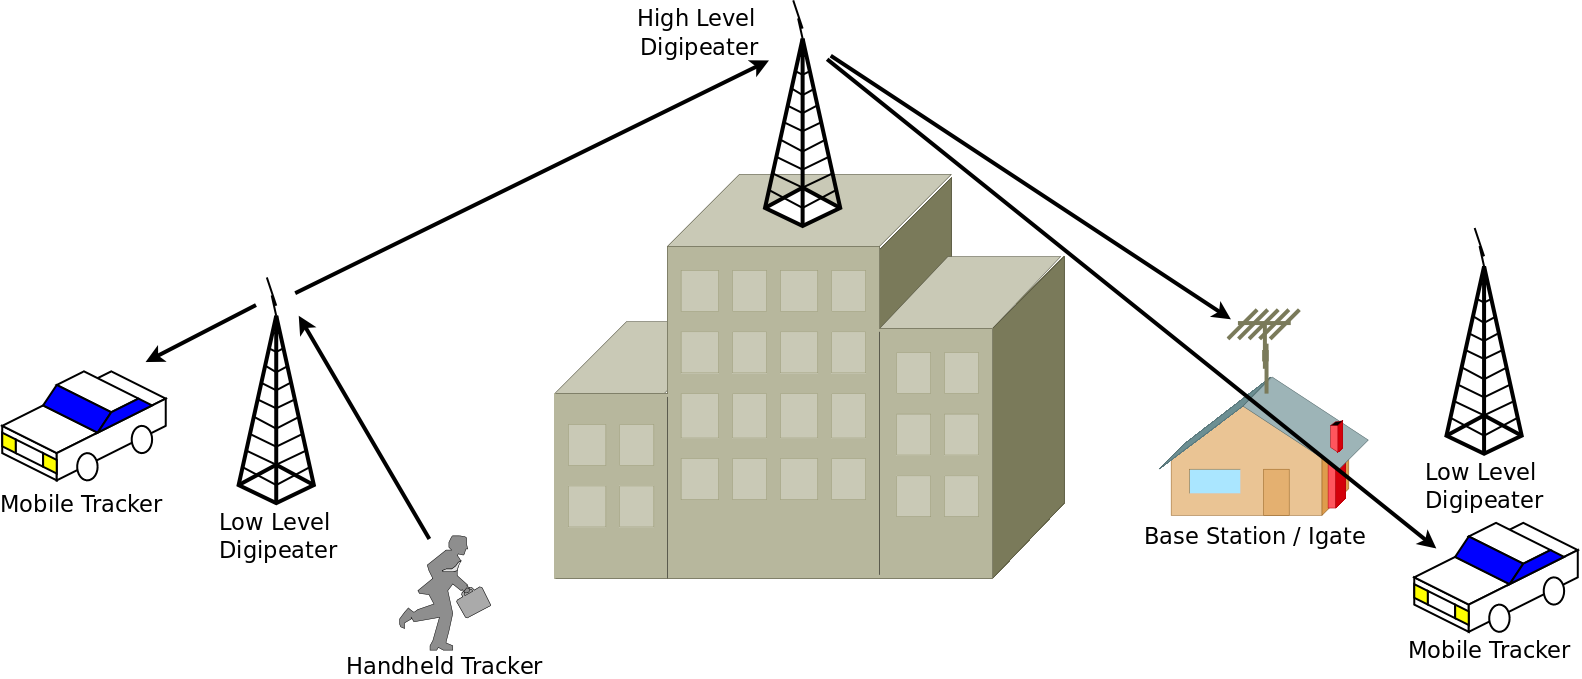
\includegraphics[width=1.0\textwidth]{src/dia/demonetwork}
	\caption{Example packet path from a handheld APRS tracker}
	\label{fig:demonetwork}
\end{figure}

\subsection{Station Block Diagrams}

Like most aspects of the APRS network, there are many options 
when assembling an APRS node.
This section presents block diagrams for the three most common ways
to assemble trackers, digipeaters, and I-gates, but additional permutations
of these and entirely different topologies are possible.

Blocks presented as dotted lines are optional. The ``Transceiver" blocks refer to 
VHF FM amateur radios. ``Terminal Node Controllers" (TNC) are the modems and radio
interfaces with minimal embedded intelligence. These blocks and the labeled protocols
between blocks will be expanded upon in later chapters.

\begin{figure}
	\centering
	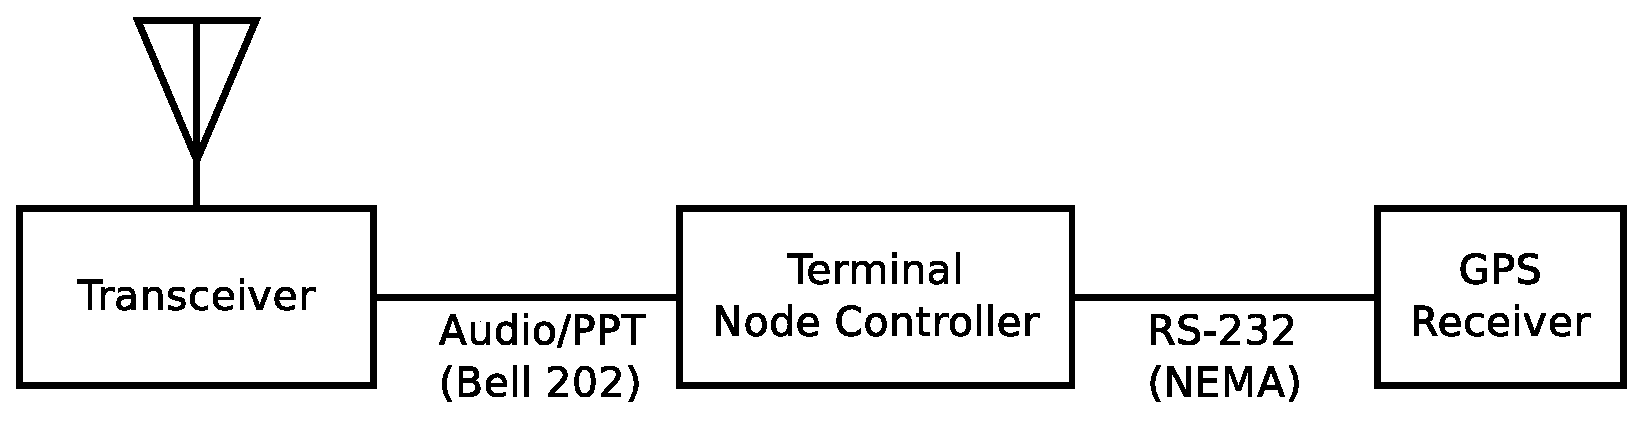
\includegraphics[width=0.7\textwidth]{src/dia/tracker}
	\caption{Block diagram for typical APRS tracker}
	\label{fig:blocktracker}
\end{figure}

Figure \ref{fig:blocktracker} shows the block diagram for an APRS tracker, 
which is built around a Terminal Node Controller which parses NEMA positions
provided by a GPS receiver and converts them into APRS position reports that
are then frequency shift modulated and sent to a VHF FM voice transceiver using an
interface cable that includes transmit and receive audio, as well as a line to
key the ``push to talk" button on the radio to start transmitting.

\begin{figure}
	\centering
	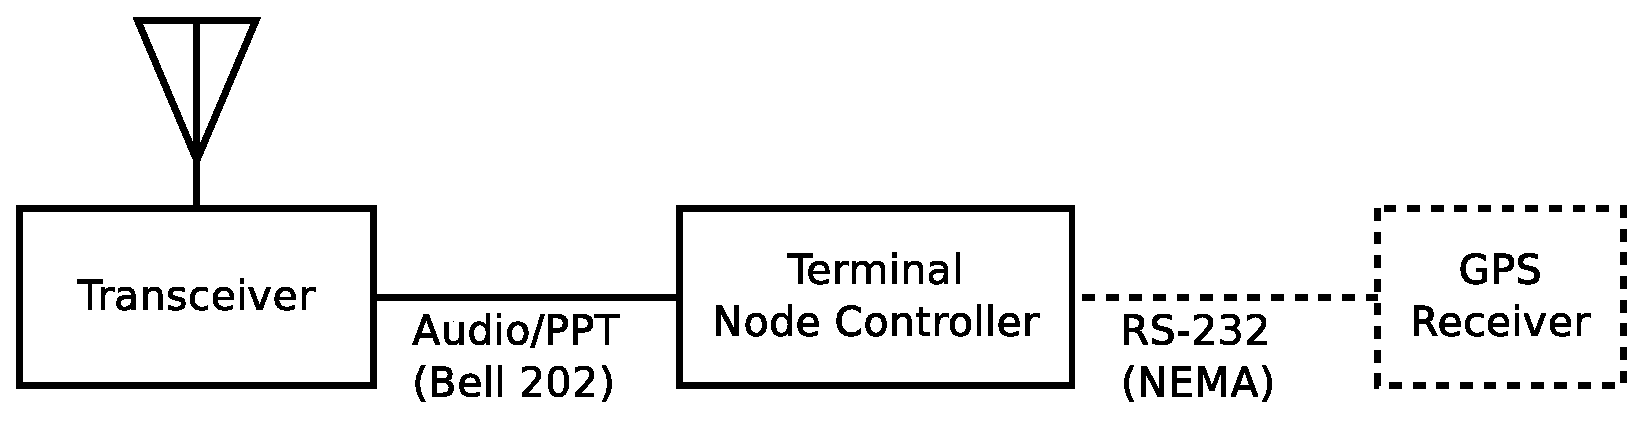
\includegraphics[width=0.7\textwidth]{src/dia/tnc_digi}
	\caption{Block diagram for typical APRS Digipeater}
	\label{fig:blockdigi}
\end{figure}

Figure \ref{fig:blockdigi} shows the block diagram for a digital repeater, which
is similar to a tracker except that the GPS receiver is often omitted. 
Since the digipeater is always installed in a fixed location, its GPS coordinates
can be hard-coded into non-volatile memory in the TNC.

\begin{figure}
	\centering
	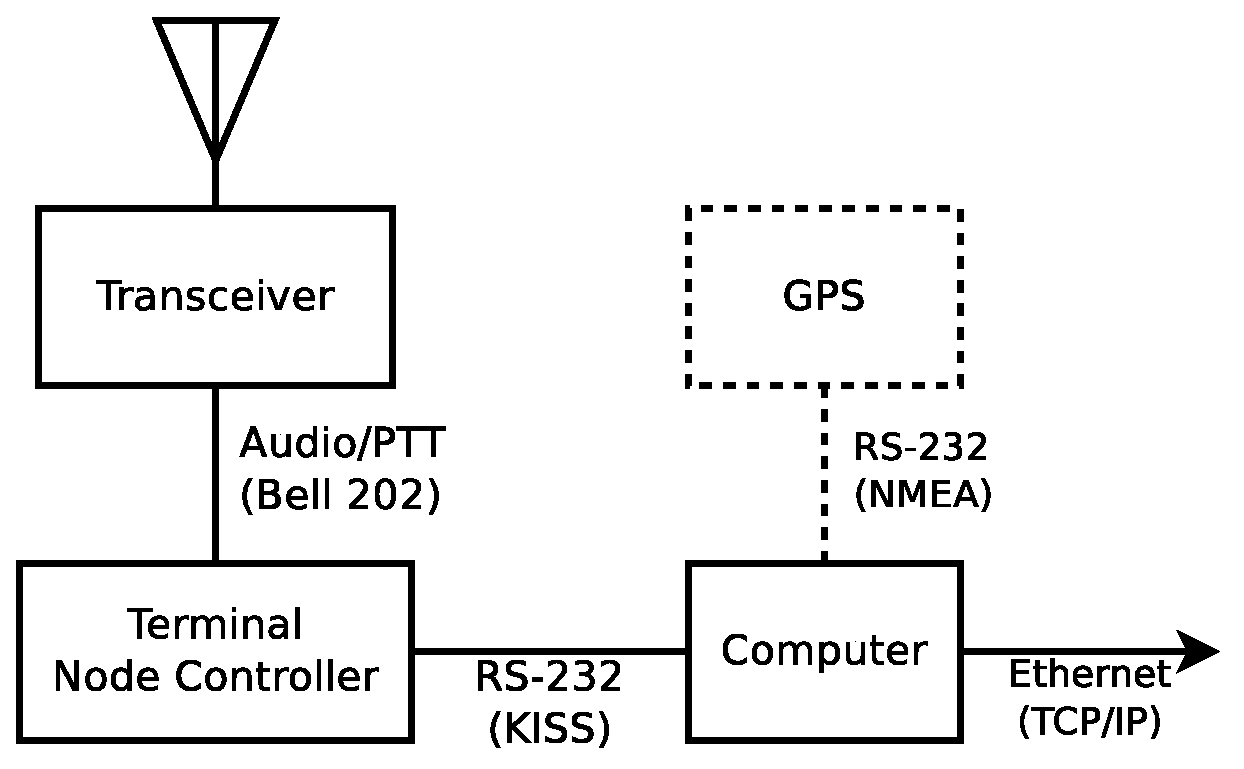
\includegraphics[width=0.7\textwidth]{src/dia/igate_kiss}
	\caption{Block diagram for typical APRS Internet Gateway}
	\label{fig:blockigate}
\end{figure}

Figure \ref{fig:blockigate} shows the block diagram for
an Internet Gateway (I-gate), which
like the digipeater doesn't require a GPS receiver. Unlike the digipeater,
instead of sending received packets back out through the VHF transceiver,
I-gates send received packets to the APRS-IS Internet System via a local connection
to the Internet.


\section{Document Overview}

The rest of this document is going to start at the bottom of the APRS protocol
stack and work its way up, touching on each layer with an introduction and
some basic analysis. 
Ideally, this document would answer all of the ambiguities existing in the
APRS network protocols, but many of the issues that will be touched upon 
deserve an entire masters thesis of their own, and therefore will often
be noted as simply deficient before moving on.

\begin{figure}
	\centering
	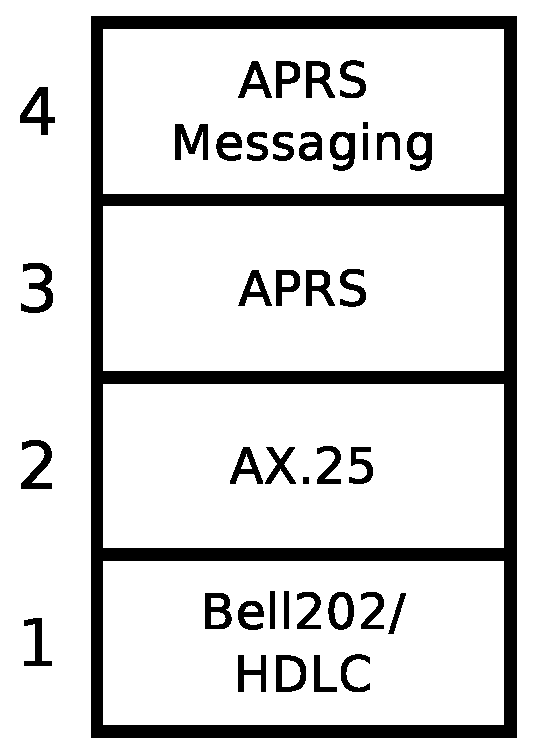
\includegraphics[width=0.4\textwidth]{src/dia/osi_full}
	\caption{The OSI network model as applied to APRS in this paper}
	\label{fig:osiaprs}
\end{figure}

The rest of this document will be divided into three parts based on the
bottom three layers of the Open Systems Interconnection (OSI) model,
to separately discuse issues found on each of these layers of the APRS network stack.
Figure \ref{fig:osiaprs} shows how the most popular protocols used on APRS
will be mapped to the OSI model, including the APRS messaging system which
will not be further mentioned due to it being a relatively unimportant part of APRS.

Part \ref{part:physical} will cover the Bell 202 modem used to encode APRS on
the VHF packet channels and the KISS protocol used to connect modems to
host devices such as computers. Chapter \ref{chap:bell202} will go into an
unusual amount of detail since a specification document for Amateur Bell 202
was never written and therefore will likely prove to be one of the more significant
contributions of this paper to the field.

Part \ref{part:datalink} will touch on what could be called the data link layer
of APRS. It will start with an introduction to the concept of a terminal
node controller, move into how the AX.25 protocol has been modified for APRS, and
finally discuss the digipeater behavior needed to flood packets from their
originating stations throughout the network.

Finally, part \ref{part:network} will discuss the popular algorithms used to 
determine how and when an individual node should send packets to the network,
and introduce some simple models for the 
expected capacity of a typical APRS network.

